\frame
{
\frametitle{}
\begin{center}
	\Huge{Características}
\end{center}
}
% Distribuciones
\frame
{
\frametitle{Distribuciones}
\begin{center}
	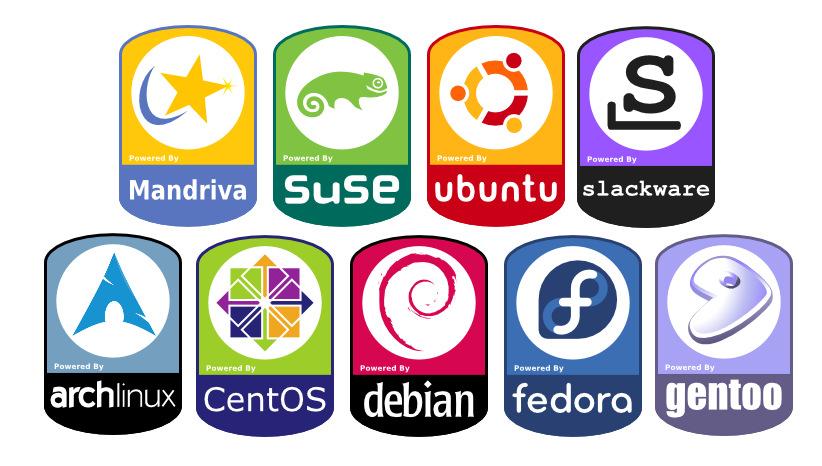
\includegraphics[width=10.5cm]{img/logos-linux}
\end{center}
}

\frame
{
\frametitle{Distribuciones}
\vspace{1cm}
\begin{center}
	
\includegraphics[width=5cm]{img/debian}
\end{center}
}

\frame
{
\frametitle{Distribuciones}
\Large{Debian}
\normalsize
\begin{itemize}
	\item El Proyecto debian es una comunidad conformada por desarrolladores y usuarios.
	\item Mantiene un sistema operativo GNU basado en software libre precompilado y empaquetado.
	\item Apuesta por separar en sus versiones el software libre del software no libre.
	\item Modelo de desarrollo ajeno a motivos empresariales o comerciales.
	\item El principal orgullo de GNU.
\end{itemize}
}

\frame
{
\frametitle{Distribuciones}
\vspace{1cm}
\begin{center}
	
\includegraphics[width=5cm]{img/redhat}
\end{center}
}

\frame
{
\frametitle{Distribuciones}
\Large{Red Hat}
\normalsize
\begin{itemize}
	\item Red Hat es la compañia responsable de la creación y mantenimiento del SO Linux \emph{Red Hat Enterprise Linux}
	\item Patrocina jboss.org y distribuye la versión profesional bajo la marca JBoss Enterprise.
	\item Uno de las principales entedidades esforzada en apoyar el movimiento del software libre.
	\item Poseen una amplia infraestructura con 2,000 empleados en 28 lugares del mundo aproximadamente.
	\item Algunas otras distribuciones basadas en Red Hat son:
	\begin{itemize}
		\item Mandriva Linux, Fedora, Yellow Dog Linux (PPC), CentOS, Scientific Linux (CERN, Fermilab LHC, ALMA)
	\end{itemize}
\end{itemize}
}

\frame
{
\frametitle{Distribuciones}
\vspace{1cm}
\begin{center}
	
\includegraphics[width=5cm]{img/ubuntu}
\end{center}
}


\frame
{
\frametitle{Distribuciones}
\Large{Ubuntu}
\normalsize
\begin{itemize}
	\item Ubuntu es una distribución Linux basda en Debian GNU/Linux.
	\item Pensada para el usuario promedio.
	\item Enfocada en la facilidad de uso.
	\item Patrocinada por Canonical Ltd. (Mark Shuttleworth)
	 \begin{itemize}
	 	\item Se financia por medio de servicios vinculados Ubuntu y soporte técnico.
	 \end{itemize}
	\item Algunas distribuciones basadas en Ubuntu son:
	\begin{itemize}
		\item Kubuntu, Xubuntu, Edubuntu y Ubuntu Server Edition
	\end{itemize}
\end{itemize}
}

\frame
{
\frametitle{Distribuciones}
\begin{center}
	
\includegraphics[width=5cm]{img/fedora}
\end{center}
}

\frame
{
\frametitle{Distribuciones}
\Large{Fedora}
\normalsize
\begin{itemize}
	\item Fedora es un SO basado en Linux, con software libre y Open Source bien actualizado.
	\item Existe una gran comunidad detrás llamada Proyecto Fedora.
	\item El Proyecto Fedora busca que sus colaboradores arreglen o contribuyan en el código del programa original, no sólo en la distribución.
	\item Es la segunda distribución más popular según DistroWatch, siendo la primera Ubuntu. 
\end{itemize}
}

\frame
{
\frametitle{Distribuciones}
\vspace{1cm}
\begin{center}
	
\includegraphics[width=6cm]{img/arch}
\end{center}
}

\frame
{
\frametitle{Distribuciones}
\Large{Arch Linux}
\normalsize
\begin{itemize}
	\item Arch Linux es una distribución GNU/Linux diseñada para ser liviana y simple.
	\item El diseño se centra en \emph{simplicidad}, \emph{elegancia}, \emph{coherencia de código} y \emph{minimalismo}.
	\item Idea central, Arch será como el usuario quiere que sea.
	\item Posee las últimas versiones de las aplicaciones y kernel.
\end{itemize}
}


% Escritorios

\frame
{
\frametitle{Entornos Gráficos}
\begin{itemize}
	\item Orientación a usuarios.
	\item Mucho más cómodo que un ambiente sólo de texto.
	\item Conjunto de elementos como:
	\begin{itemize}
		\item Ventanas
		\item Iconos
		\item Barras de herramientas
	\end{itemize}
\end{itemize}
}

\frame
{
\frametitle{Entornos Gráficos}
\Large{GNOME}
\begin{columns}
	\begin{column}{0.2\textwidth}
		
\includegraphics[width=3cm]{img/gnome-logo}
	\end{column}
	\begin{column}{0.8\textwidth}
		\begin{center}
			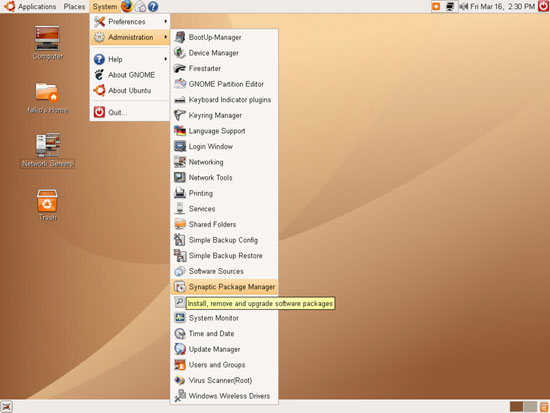
\includegraphics[width=8cm]{img/gnome}
		\end{center}
	\end{column}
\end{columns}
}

\frame
{
\frametitle{Entornos Gráficos}
\Large{KDE}
\begin{columns}
	\begin{column}{0.2\textwidth}
		
\includegraphics[width=3cm]{img/kde-logo}
	\end{column}
	\begin{column}{0.8\textwidth}
		\begin{center}
			
\includegraphics[width=8cm]{img/kde}
		\end{center}
	\end{column}
\end{columns}
}

\frame
{
\frametitle{Entornos Gráficos}
\Large{LXDE}
\begin{columns}
	\begin{column}{0.2\textwidth}
		
\includegraphics[width=3cm]{img/lxde-logo}
	\end{column}
	\begin{column}{0.8\textwidth}
		\begin{center}
			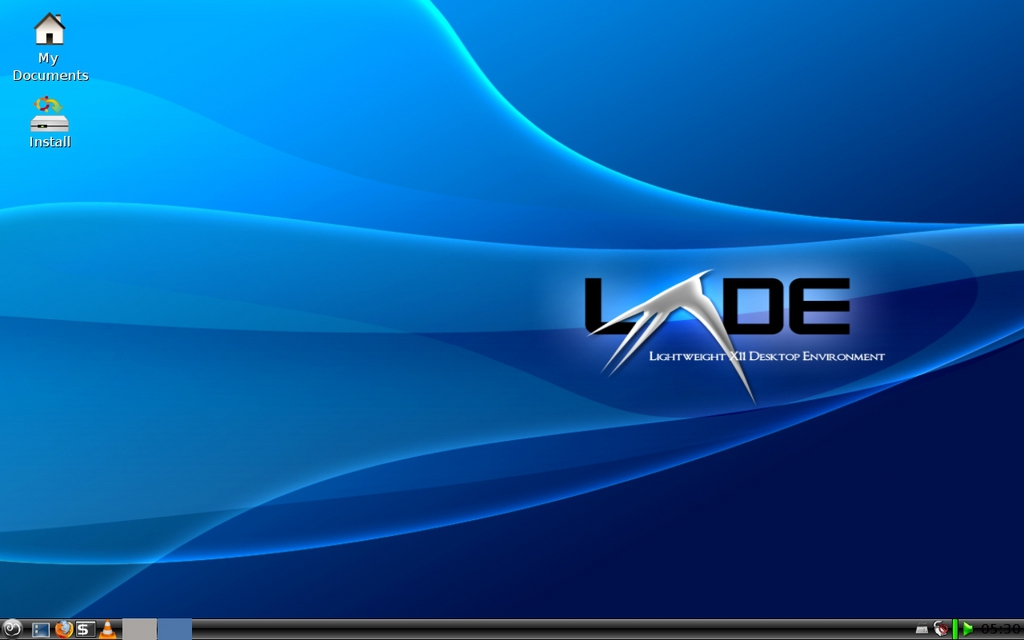
\includegraphics[width=8cm]{img/lxde}
		\end{center}
	\end{column}
\end{columns}
}

\frame
{
\frametitle{Entornos Gráficos}
\Large{XFCE}
\begin{columns}
	\begin{column}{0.2\textwidth}
		
\includegraphics[width=3cm]{img/xfce-logo}
	\end{column}
	\begin{column}{0.8\textwidth}
		\begin{center}
			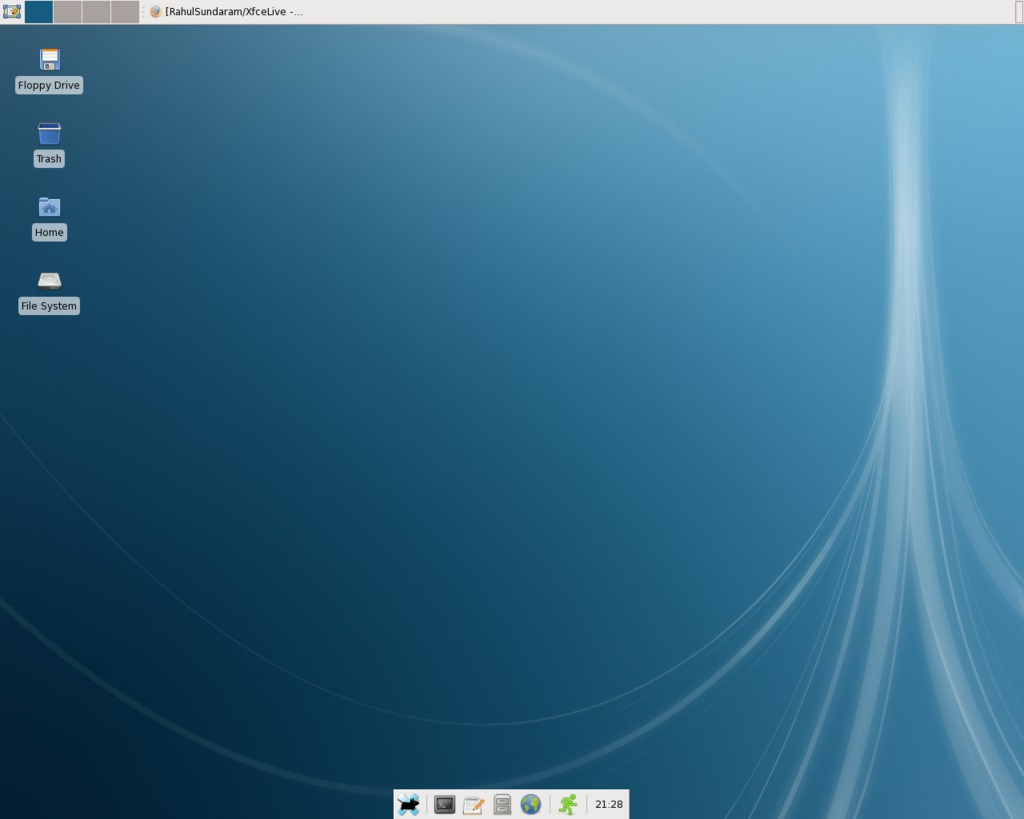
\includegraphics[width=8cm]{img/xfce}
		\end{center}
	\end{column}
\end{columns}
}

\frame
{
\frametitle{Entornos Gráficos}
\begin{itemize}
	\item Existen varios entornos gráficos aparte de los nombrados.
	\item ...y que no son malos ni nada por el estilo.
	\begin{itemize}
		\item FluxBox, BlackBox, OpenBox, Enlightenment, WindowsMaker, IceWM, FVWM, etc.
	\end{itemize}
\end{itemize}
}

\frame
{
\frametitle{Modelo de Desarrollo}
\begin{itemize}
	\item El paradigma Cliente/Usuario no se cumple del todo.
	\begin{itemize}
		\item Colaboraciones internacionales
		\item Cualquier persona puede arreglar un bug de un programa importante
	\end{itemize}
	\item Todos pueden participar.
\end{itemize}
}


